\documentclass[a4paper, 10pt]{cesenaexam}
\usepackage[T1]{fontenc}
\usepackage[utf8]{inputenc}
%\usepackage{lmodern}
\usepackage[italian]{babel}
\usepackage{booktabs}
\usepackage{cite}
\graphicspath{{./images/}}
\usepackage{amsfonts, amssymb, amsmath, textcomp, gensymb, mathtools}
\interdisplaylinepenalty=2500
\usepackage{array}
\usepackage{url}
\usepackage{microtype, datetime}
\usepackage{color, soul}
\usepackage[capitalise]{cleveref}
\usepackage{siunitx}

\newcommand{\R}{\mathbb{R}}
\newcommand{\C}{\mathbb{C}}
\renewcommand{\Re}{\operatorname{Re}}
\renewcommand{\Im}{\operatorname{Im}}

%%
% Set the title and parts here
%%
\title{\bf Elettrotecnica - Ing. Aerospaziale, Ing. Meccanica \\
    \bf A.A. 2016/17 - Prova n.3 - 21 luglio 2017}

\examparts{\bfseries Parti Svolte: \hspace{1cm}%
    E1 \boxempty \hspace{1cm}%
    E2 \boxempty \hspace{1cm}%
    D \boxempty}

\begin{document}
\maketitle{Cognome}{Nome}{Matricola}{Firma}{1}

\examsection*{Esercizio 1}{11 punti}
\examtwoblocks{0.385\textwidth}{0.58\textwidth}{
\begin{tikzpicture}
\draw (0,0)
node [label={below:$D$}] {} 
to [short, *-] ++(2.5,0)
to [R, l=$R_4$, i_=$I_4$] ++(0,3)
node [label={right:$C$}] {} coordinate (C)
-- ++(0,1.5)
to [controlled voltage source, v_=$\mu V_4$] ++(-5,0)
-- ++(0,-1.5)
node [label={left:$A$}] {} coordinate (A)
to [short, *-, i={\relax}] ++(0.5,0) ++(-0.5,0)
to [R, l=$R_1$, -*] ++(2.5,0)
node [label={above:$B$}] {} coordinate (B)
to [controlled current source, l=$\alpha I_4$, i_={\relax}, -*] ++(2.5,0)
;
\draw (0,0)
to [V, v_=$V_{G3}$] ++(0,1.5)
to [R, l=$R_3$] ($(B) - (0,0.5)$)
to [short, i<={\relax}] (B)
;
\draw (0,0)
-- ++(-2.5,0)
to [R, l=$R_2$, i={\relax}] (A)
;
\end{tikzpicture}
}{%
Supponendo noti i parametri dei componenti, illustrare il procedimento di risoluzione del circuito rappresentato in figura con il {\bf metodo delle tensioni di nodo}:%
\begin{enumerate}
\item indicare quali grandezze vengono scelte come incognite del sistema risolvente;
\item scrivere le espressioni della matrice dei coefficienti e del vettore dei termini noti del sistema risolvente;
\item scrivere le espressioni in funzione delle incognite indicate al punto 1 delle correnti dei resistori;
\item scrivere le espressioni in funzione delle incognite e delle correnti determinate al punto 3 delle potenze erogate dai generatori.
\end{enumerate}%
}

\examsection*{Esercizio 2}{11 punti}
\examtwoblocks{0.65\textwidth}{0.32\textwidth}{
\begin{tikzpicture}
\draw (0,0) coordinate (ref)
to [V, v=$V_G$] ++(0,1.5)
to [ european resistor, l=$\mathbf{Z}_G$] ++(0,1.5) coordinate (topZG)
-- ++(1.5,0) coordinate (T1top)
(T1top |- 0,0) coordinate (T1bot)
-- (0,0)
;
\newlength{\myRT}\pgfmathsetlength{\myRT}{0.5cm} 
\coordinate (T2bot) at ($(1.8,0) + (0.8*\myRT,0)$);
\coordinate (T2top) at (T2bot |- 0,3);
\draw (T1bot)
-- ($(T1bot)!0.5!(T1top) - (0,\myRT)$) coordinate (T1mtop);
\draw (T2bot)
-- ($(T2bot)!0.5!(T2top) - (0,\myRT)$) coordinate (T2mtop);
\draw [thick] (T1mtop)
arc [start angle=-90, end angle=90, radius=\myRT] coordinate (T1ptop);
\draw [thick] (T2mtop)
arc [start angle=-90, end angle=-270, radius=\myRT] coordinate (T2ptop);
\node (Tname) [anchor=south] at ($(T1ptop) + (0.8\myRT,0)$) {$k$};
\draw (T1ptop) to (T1top);
\draw (T2ptop) to (T2top);
\draw (T2top)
to [european resistor, l=$X$] ++(2,0) coordinate (Xright);
\draw (Xright)
-- ++(0,0.5) 
to [short,i>^=$i_1$] ++(0.5,0)
to [R, l=$R_1$] ++(1,0)
to [L, l=$L_1$] ++(1.5,0)
-- ++(0,-1)
to [controlled current source, i<=\relax, l=$\alpha i_1$] ++(-3,0)
to [short, -*] (Xright)
;
\draw ($(Xright)+(3,0)$)
to [short, *-] ++(1,0)
to [short, -*] ++(0,-0.5) coordinate (R2C2centop)
to [short] ++(0.5,0)
to [C, l_=$C_2$] ++(0,-2)
to [short] ++(-1.3,0)
to [R, l=$R_2$] ++(0,2)
-- ++(0.8,0)
;
\draw (T2bot)
-- (T2bot -| R2C2centop)
to [short, -*] ++(0,0.5)
;
\draw ($(T2bot) + (0,0.5)$)
to [open, v=$v$] ($(T2bot) + (0,2.5)$);
\draw [dashed] ($(Xright) + (-0.2,1.4)$) rectangle (9.2,-0.2);
\end{tikzpicture}
}{\begin{tabular}{ll}%
$R_1 =$ \SI{4}{\ohm} & $L_1 =$ \SI{4}{mH} \\
$R_2 =$ \SI{20}{\ohm} & $C_2 =$ \SI{100}{\mu F} \\  
$\alpha =$ \si{3} \\
\multicolumn{2}{l}{$V_G =$ $\mathrm{120\sqrt{5} \cos(\omega t + \phi)}$ \si{V}} \\
$\cos \phi = \mathrm{\sqrt{5}/5}$ & $\sin \phi = \mathrm{-2\sqrt{5}/5}$ \\
$\omega =$ \SI{100}{rad/s} \\
\multicolumn{2}{l}{$\mathbf{Z}_G = \mathrm{180 + 180j}$ \si{\ohm}}
\end{tabular}%
}
Il circuito rappresentato in figura è in condizioni di regime sinusoidale. Determinare:
\begin{enumerate}
\item l’impedenza equivalente, $\mathbf{Z}_{eq}$, del bipolo racchiuso dalla linea tratteggiata;
\item la potenza disponibile, $P_d$, del bipolo formato dal generatore $V_G$ e dall’impedenza $\mathbf{Z}_{G}$;
\item i valori da attribuire al rapporto di trasformazione $k$ e alla reattanza $X$ affinché la potenza attiva assorbita da $\mathbf{Z}_{eq}$ sia uguale a $P_d$;
\item l’espressione della tensione $v(t)$ (con i valori di $k$ e $X$ determinati al punto precedente).
\end{enumerate}

\newpage
\examsection*{Domande}{10 punti}
\begin{enumerate}
\item \examtwoblockstop{9cm}{6cm}{
    \begin{tikzpicture}
    \node (text) [align=justify, text width=0.97\textwidth] {%
    Le tensioni concatenate costituiscono una terna diretta di valore efficace \SI{866}{V}.
    Determinare il valore efficace $I$ delle correnti di linea e il valore efficace $I_{\Delta}$ delle correnti nei resistori $R_2$. (\textit{2 punti})\\
    $R_1 =$ \SI{5}{\ohm}, $R_2 =$ \SI{30}{\ohm}, $\omega L =$ \SI{10}{\ohm}.
    };
    \node (I) [draw, anchor=north west, minimum width=1cm, minimum height = 1cm] at (text.south west) {$I$};
    \node (I box) [draw, anchor=north west, minimum width=3cm, minimum height = 1cm] at ($(I.north east)+(-\pgflinewidth,0)$) {};
    \node (Idelta) [draw, anchor=north west, minimum width=1cm, minimum height = 1cm] at ($(I box.north east)+(-\pgflinewidth,0)$) {$I_{\Delta}$};
    \node (Idelta box) [draw, anchor=north west, minimum width=3cm, minimum height = 1cm] at ($(Idelta.north east)+(-\pgflinewidth,0)$) {};
    \end{tikzpicture}%
    }{%
    \begin{tikzpicture}[scale=0.7, transform shape]
    \draw (0,0)
    node [label={left:$1$}] {}
    to [short, *-, i=\relax] ++(1,0)
    to [R, l=$R_1$] ++(1,0) coordinate (L1p)
    -- ++(2.5,0) coordinate (R21)
    to [R, l=$R_2$, *-] ++(2,0) coordinate
    -- ++(0,-0.5) coordinate (R21p)
    to [short, i=\relax] (R21p -| R21)
    to [short, -*] ++(0,-1) coordinate (R22)
    to [R, l=$R_2$, *-] ++(2,0)
    -- ++(0,-0.5) coordinate (R22p)
    to [short, i=\relax] (R22p -| R22)
    to [short, -*] ++(0,-1) coordinate (R23)
    to [R, l=$R_2$, *-] ++(2,0)
    -- ++(0.5,0)
    to [short, i=\relax] ++(0,4)
    -- ++(-2.5,0)
    -- ++(0,-1)
    ;
    \draw (R22)
    -- ++(-2.5,0)
    to [R, l_=$R_1$] ++(-1,0)
    to [short, i<=\relax, -*] ++(-1,0)
    node [label={left:$2$}] {}
    ;
    \draw (R23)
    -- ++(-2.5,0)
    to [R, l_=$R_1$] ++(-1,0)
    to [short, i<=\relax, -*] ++(-1,0)
    node [label={left:$3$}] {}
    ;
    \draw ($(L1p)!0.1!(R21)$)
    to [short, *-] ++(0,-3.5)
    to [L, l_=$L$] ++(0,-1)
    -- ++(0,-0.5) coordinate (L1m)
    ;
    \draw ($(L1p)!0.5!(R21) + (0,-1.5)$)
    to [short, *-] ++(0,-2)
    to [L, l_=$L$] ++(0,-1)
    -- ++(0,-0.5) coordinate (L2m)
    ;
    \draw ($(L1p)!0.9!(R21) + (0,-3)$)
    to [short, *-] ++(0,-0.5)
    to [L, l_=$L$] ++(0,-1)
    -- ++(0,-0.5) coordinate (L3m)
    ;
    \draw (L1m)
    to [short, -*] (L2m)
    -- (L3m)
    ;
    \end{tikzpicture}}
\item \examtwoblockstop{10cm}{5cm}{
    \begin{tikzpicture}
    \node (text) [align=justify, text width=0.97\textwidth] {%
    Per $t<0$ il circuito è in condizioni di regime stazionario e l’interruttore è chiuso.
    All’istante $t=0$ si apre l’interruttore.
    Determinare l’espressione di $i_{L}(t)$ per $t>0$.
    (\textit{2 punti})
    };
    \node (iL) [draw, anchor=north west, minimum width=1cm, minimum height = 1cm] at (text.south west) {$i_{L} (t)$};
    \node (iL box) [draw, anchor=north west, minimum width=7cm, minimum height = 1cm] at ($(iL.north east)+(-\pgflinewidth,0)$) {};
    \end{tikzpicture}%
    }{%
    \begin{tikzpicture} [scale=0.8, transform shape]
    \draw (0,0) coordinate (circuit north west)
    to [short, -*] ++(0,-1)
    to [R, l=$R$] ++(0,-2)
    -- ++(2,0)
    to [short, *-] ++(2,0)
    to [L, -*, i_<=$i_L$, l=$L$] ++(0,2)
    to [R, -*, l_=$R$] ++(-2,0) coordinate (IGp)
    to [R, -*, l_=$R$] ++(-2,0);
    \draw (IGp) to [I, i<=\relax, l=$I_G$] ++(0,-2);
    \draw (circuit north west)  -- ++(1.5,0) coordinate (Swm);
    \coordinate (Swp) at ($(Swm)+(1,0)$);
    \draw (Swp)
    -- ++(1.5,0)
    -- ++(0,-1)
    ;
    \node [circ] at (Swm){};
    \node [circ] at (Swp){};
    \draw [thick] (Swm) -- (Swp);
    \draw [densely dotted,thin] let \p1 = ($(Swp)-(Swm)$) in (Swm) -- ++(30:({veclen(\x1,\y1)}););
    \coordinate (Swmiddown) at ($(Swm)!0.5!(Swp) + (0,-0.2)$);
    \draw [->, switcharc] (Swmiddown) arc [start angle=-10, end angle=60, radius=0.6cm];
    \end{tikzpicture}}
\item \examtwoblockstop{11cm}{4cm}{
    \begin{tikzpicture}
    \node (text) [align=justify, text width=0.97\textwidth] {%
    Il carico trifase rappresentato nella figura viene alimentato mediante una terna simmetrica di tensioni concatenate.
    Se la potenza assorbita quando l’interruttore è chiuso è $P_c =$ \SI{3}{\kW}, qual è la potenza $P_a$ assorbita con l’interruttore aperto? (\textit{2 punti})
    };
    \node (Pa) [draw, anchor=north west, minimum width=1cm, minimum height = 1cm] at (text.south west) {$P_{a}$};
    \node (Pa box) [draw, anchor=north west, minimum width=7cm, minimum height = 1cm] at ($(Pa.north east)+(-\pgflinewidth,0)$) {};
    \end{tikzpicture}
    }{
    \begin{tikzpicture}[scale=0.8, transform shape]
    \draw (0,0)
    node [label={left:$1$}] {}
    to [short, *-, i=\relax] ++(1,0) coordinate (R1p);
    \draw (0,1.5)
    node [label={left:$2$}] {}
    to [short, *-, i=\relax] ++(1,0) coordinate (R2p);
    \draw (0,3)
    node [label={left:$3$}] {}
    to [short, *-, i=\relax] ++(1,0) coordinate (R3p);
    \draw (R1p)
    to [short] ++(0.5,0)
    to [R, l=$R$] ++(1,0)
    to [short] ++(0.5,0)
    to [short, -*] ++(0,1)
    ;
    \draw (R2p)
    to [short, *-] ++(0,0.5)
    -- ++(0.5,0)
    to [R, l=$2R$] ++(1,0)
    to [short] ++(0.5,0) 
    -- ++(0,-0.2) coordinate (Swm)
    ;
    \draw (R2p)
    to [short] ++(0,-0.5)
    -- ++(0.5,0)
    to [R, l=$2R$] ++(1,0)
    to [short] ++(0.5,0) 
    -- ++(0,+0.2) coordinate (Swp)
    ;
    \draw (R3p)
    to [short] ++(0.5,0)
    to [R, l=$R$] ++(1,0)
    to [short] ++(0.5,0)
    to [short, -*] ++(0,-1)
    ;
    \node [circ] at (Swm){};
    \node [circ] at (Swp){};
    \draw [thick] (Swm) -- (Swp);
    \draw [densely dotted] let \p1 = ($(Swp)-(Swm)$) in (Swm) -- ++(-60:({veclen(\x1,\y1)}););
    \coordinate (Swmiddown) at ($(Swm)!0.5!(Swp) + (-0.1,0)$);
    \draw [->, switcharc] let \p1 = ($(Swp)-(Swm)$) in (Swmiddown) arc [start angle=-100, end angle=-45, radius=({veclen(\x1,\y1)})];
    \end{tikzpicture}
    }
\item \examtwoblockstop{11cm}{5cm}{
    \begin{tikzpicture}
    \node (text) [align=justify, text width=0.97\textwidth] {%
    Si considerino due avvolgimenti di $N_1$ e $N_2$ spire disposti su un nucleo toroidale avente raggio medio $r$ e sezione $S$.
    Se il raggio $r$ viene raddoppiato, è possibile mantenere invariato il coefficiente di mutua induzione dei due avvolgimenti: (\textit{1 punto})
    };
    \node (choices) [anchor=north west, text width=0.97\textwidth] at (text.south west) {%
    $\square \;$ dimezzando il numero di spire di entrambi gli avvolgimenti\\
    $\square \;$ raddoppiando il numero di spire di entrambi gli avvolgimenti\\
    $\square \;$ raddoppiando il numero di spire di uno degli avvolgimenti\\
    $\square \;$ raddoppiando il valore delle correnti nei due avvolgimenti};
    \end{tikzpicture}
    }{
    \begin{tikzpicture}
    \node (image) {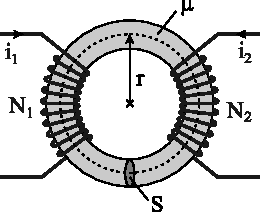
\includegraphics[width=0.9\textwidth]{toroid_mutual}};
    \end{tikzpicture}
    }
\item \examoneblocktop{15cm}{
    \begin{tikzpicture}
    \node (text) [align=justify, text width=0.97\textwidth] {%
    L’area racchiusa da un ciclo di isteresi nel piano H-B corrisponde: (\textit{1 punto})
    };
    \node (choices) [anchor=north west, text width=0.97\textwidth] at (text.south west) {%
    $\square \;$ alla potenza dissipata in un ciclo di isteresi\\
    $\square \;$ alla densità volumetrica di energia dissipata in un ciclo di isteresi\\
    $\square \;$ all’energia accumulata nel campo magnetico in un ciclo di isteresi};
    \end{tikzpicture}
    }
\item \examoneblocktop{15cm}{
    \begin{tikzpicture}
    \node (text) [align=justify, text width=0.97\textwidth] {%
    In condizioni di risonanza il fattore di potenza di un bipolo RLC serie è: (\textit{1 punto})
    };
    \node (choices) [anchor=north west, text width=0.97\textwidth] at (text.south west) {%
    $\square \;$ nullo\\
    $\square \;$ minimo\\
    $\square \;$ massimo};
    \end{tikzpicture}
    }
\item \examoneblocktop{15cm}{
    \begin{tikzpicture}
    \node (text) [align=justify, text width=0.97\textwidth] {%
    Il valore medio della potenza istantanea reattiva assorbita da un bipolo passivo in regime sinusoidale: (\textit{1 punto})
    };
    \node (choices) [anchor=north west, text width=0.97\textwidth] at (text.south west) {%
    $\square \;$ è sempre $\geq$ 0 \\
    $\square \;$ è sempre $\leq$ 0 \\
    $\square \;$ è sempre nullo \\
    $\square \;$ è $\geq$ 0 per i bipoli RL e $\leq$ 0 per i bipoli RC};
    \end{tikzpicture}
    }
\end{enumerate}
\end{document}